\documentclass[11pt]{article}
\usepackage{setspace}
\usepackage{titling}
\usepackage[a4paper,margin=1in]{geometry}
\usepackage{enumitem}
\usepackage{fancyhdr}
\usepackage{titlesec}
\usepackage{ebgaramond}
\usepackage[T1]{fontenc}
\usepackage{hyperref}
\usepackage{graphicx}
\usepackage{float}

\renewcommand{\thesection}{\Roman{section}.}
\renewcommand{\thesubsection}{\alph{subsection}.}
\renewcommand{\thesubsubsection}{\thesubsection\roman{subsubsection}}

\hypersetup{
  colorlinks=true,
  linkcolor=blue,
  urlcolor=blue
}

% --- header ---
\pagestyle{fancy}
\fancyhf{}
\fancyhead[L]{Department of Computer Science \\
  \rule[-2ex]{0pt}{2ex}Ateneo de Naga University}
\vspace{5cm}
\fancyfoot[C]{\thepage}

\setlength{\headheight}{30pt}
\setlength{\headsep}{20pt}

\begin{document}

% --- cover page ----
\begin{titlepage}
  \thispagestyle{fancy}
  
  \vspace*{4cm}
  \centering
  \vfill
  {\LARGE \textbf{REVIVERS}} \\
  \vspace{0.5cm}
  CSMC311 Software Engineering 2 \\
  Proposal Paper
  
  \vfill
  
  \textbf{Game Designer, Programmer, Project Manager} \\
  Jonel C. Ganalon -- N2
  
  \vspace{1cm}
  
  \vfill 
\end{titlepage}

\tableofcontents
\newpage
\listoffigures
\newpage
\listoftables
\newpage

\section{Introduction}
\subsection{Overview}
Revivers is a prospective open-source turn-based strategy game revolving around the use of languages to reclaim territories overrun by foreign people. The players of the game lead the Revivers aiming to overthrow the foreign government, the Imperial Government, occupying their land. Revivers discovered a powerful way to fight the Imperalists using their already lost native language. They discovered that their native language has power over anything on their land. However, the Imperialists ruined every source of their native language and compeled everyone to use their Imperial language instead. The role of the players come into play as those who still have the knowledge of the lost native language. The players must gather allies from the people and help bring back their culture, identity, and home from the foreign occupants.


\subsection{Purpose of the Application}
The game provides a platform for documenting languages. The game contains specimens from real-life languages that the player must discover to unlock gameplay elements. Aside from that, players themselves contribute to this purpose by collecting real life words from their chosen language and inputting them into the game. This involves everyone in saving their own languages from possible threats of extinction in the future. This is particularly relevant in the Philippines, where documentation of local languages receives little attention. Furthermore, the game encourages lexical innovation (a linguistic process where new words of terms enter a language) and touches linguistic purism as it rewards words constructed using neologism.

\subsection{Objectives}
The objectives of the project are as follows:

\begin{itemize}
    \item Document at least 200 native words in the prototype to promote language preservation.
    \item Implement a functional turn-based system that allows players to perform actions per turn.
    \item Design and implement the core gameplay loop using an Entity–Component–System (ECS) architecture to ensure modularity and scalability.
    \item Develop basic language revival mechanics, including recruiting and reclaiming actions.
    \item Implement NPC behavior and interactions using AI-driven systems for allies, neutral citizens, and opponents.
    \item Create a functional map of the game area with tile-based movement and territorial control.
    \item Design and integrate key game attributes such as health, mana, hunger, insight, and prestige.
    \item Implement the stage progression system based on the eight stages of language revival as per Joshua Fishman’s model.
    \item Develop a basic user interface for action selection, resource tracking, and event feedback.
    \item Enable save/load functionality to preserve player progress and dictionary entries.
    \item Conduct iterative testing and playtesting to refine mechanics, balance resources, and ensure gameplay is engaging.
\end{itemize}

\subsection{Game Specifics}
\subsubsection{Game Theme}
The game will be visually similar to Civilisation or Freeciv. It will also be more text-based.
\begin{itemize}
\item
  Cultural Preservation/Language Revival
\item
  Education/Learning
\item
  Exploration/Discovery
\item
  Identity/Connection
\end{itemize}

\subsubsection{Game Genres}
\begin{itemize}
\item
  Educational
\item
  Adventure
\item
  Role-playing
\item
  Turn-Based Strategy
\end{itemize}
  
\subsubsection{Gameplay and Mechanics}
For the prototype of the game, the game will use English as the Imperial language and Bicol Naga as the native language. As the game starts for the first time, it will ask for the username of the players. It will reveal that the players have awaken from a dream. Then, the players' character (MC will then proceed to demonstrate its dream as the gameplay of the game, revealing it as the guidance from the spirit of their lost language. During the game, the players will input Bicol root words into the game storing it in their own dictionary.\\
The players will play on a pre-defined map adapted from the real-life map of Naga City. The Imperium controls most of the map especially important buildings like Hospitals, Universities, and Governmental ones. There is also the Imperial Police (IP) that patrols around the map and checks every buildings to look for Revivers. The game is turn-based and a turn can be made once the players made an action. Actions require arguments and these are any entities on the game. Actions are basically the verbal roots that the players input into the game and the arguments are the nominal roots that the players input into the game plus the already existing entities on the game's map such as the buildings. Using the words that the players own, they will make sentences that will drive the game.\\

\textbf{Entity Markers}\\
Entities refer to objects in the game that are nouns. In order to use these nouns, the players must choose the correct noun markers for them. There are three sets of markers in Bicol: the \textbf{si}-markers, \textbf{ki}-markers, and \textbf{sa-markers}.\\
The \textbf{si} set of markers:\\
\textbf{si}: This is used for entities with personal names such as allies whom the players have given names, a Reviver. This will make the entity the focus of the action.
\textbf{an}: Similar to \textbf{si} but is used for common nouns.\\
The \textbf{ni} set of markers are the non-focus arguments of a verb. They are the following:\\
\textbf{ni}: This is used to refer to entities with personal names.\\
\textbf{nin}: This is used to refer to entities that are common or general.\\
The \textbf{locative} markers refer to a place or direction of an action. They are the following:\\
\textbf{ki}: This is used for entities with personal names.\\
\textbf{sa}: This is used for entities that has common or general names.\\
Another set of markers also exist. They are the personal pronouns of Bicol.\\

\textbf{Action}\\
Once a marker is chosen for specific entity, it will hover above that entity. The players can then select an action from the verbal roots. After this, the players must correctly conjugate the verb by selecting affixes that marks the \textbf{role} of the focused entity and the \textbf{aspect} of the verb.
\textbf{-in-}: This affix signify that the role of the focused entity is the receiver or patient of the action.\\
\textbf{-nag-}: This affix signifiy that the role of the focused entity is the actor of the action.\\
\textbf{-in-an}: This affix signify that the role of the focused entity is the place of the action.\\
\textbf{perfective}: This aspect means that the action has been finished. This action only persists at each turn of the player. The action finished once the turn is done.
\textbf{imperfective}: This aspect means that the action has not yet finished. This action continues up to the next turn in the game.
\textbf{contemplative}: This aspect means that the action is yet to be done. This action will happen in the next turn of the game.\\
The choices of the players are crucial since this can make an action target the enemy or target themselves or their allies.\\

The simplest task of the players is to avoid the patrolling IP by moving places. This can be done by selecting the MC, marking it as \textit{kami} to include the other Revivers, selecting the verbal root \textit{duman} and using \textit{nag-}, selecting a place like a tile on the map or a building and marking it as \textit{sa}, then making a turn.\\

\textbf{Food}\\
Food is crucial in the game. Food lets the Revivers recruit people or reclaim people. This is one of the players tasks in the game. Food can be obtained in the forest sections of the map or from buildings that produces kinds of food. The players give food to the Revivers so that they can recruit people. Revivers are people that are part of a group like in professions that is why they are tasked to recruit people.\\

\textbf{Conversion Chains}\\
When a building is reclaimed, the neighbouring households can be converted to allies or speaker of the language given that enough food is avaible.\\

\textbf{Pushback Mechanics}\\
In every stage of the game, there is a limit to how speed conversions happen, if the players exceed this limit, it will trigger checking from the Imperial Police.\\

\textbf{Insight}\\
Every people in the game has an attribute called Insight. Players need this to input words into the game. The more people the players recruit as ally, the more Insights they will have. Different kind of words will have different number of Insight requirement.\\

\hypertarget{prestige}{\textbf{Prestige}}\\
Prestige  is the meter on how powerful the language is. The more words the language has the higher its prestige. Prestige adds multipler to the damages of the players attacks using the words. For example, \textit{machete} and \textit{sundang} both have the same base damage, but in actuality, they can differ in damage. The language with the higher prestige will have the higher damage output. This is why expanding the language is important.\\

\textbf{Nouns}\\
Every entity in the game has its corresponding nouns. Knowing the nominal names give the players power over that entity. For example, in order to use wood, the player must record the Bicol word kahoy. Nouns reffering to objects have damage attributes. They have varying amount of damage depending on object. For example, sundang has higher damage than tukawan.
There are also nouns referring to places. These nouns can reclaim building institutions in the game like entering the Bicol word for hospital will give players access to it.

Derivation is the process of adding affixes to nouns to create new words. Bicol has several productive ways of doing derivations. Aside from this, players can do neologism. Neologism is where the player creates new word that does not exist in the Bicol language. Doing neologism costs more Insights but sometimes provides additional benefits. It adds more \hyperlink{prestige}{Prestige} to the language.

The following are the possible \textbf{affixes} in the game:\\


\textbf{Verbs}\\
Verbal words give players actions. Learning an action takes time and different actions can have varying needed duration to be learned. Verbs are divided into transitive and intransitive. Transitive verbs require at least two arguments: the actor and the patient; while Intransitive verbs require at least one argument, the actor or the patient.\\

\textbf{Defence}\\
Defence is an attribute that each institutions or buildings has. The defence increases with the number of native words associated to that institution.\\

\textbf{Combats}\\
There are several combats in the game implemented using turn-based strategy.\\
\textbf{Physical Objects}:
Imperials and the players can fight using physical objects. The damage of the physical object can be increased during fights by using \textbf{semantic chaining}. The enemy or the players provide words related to their weapon. The more words provided, the stronger the attack. This means that bigger vocabulary can offer longer semantic chains.\\
\textbf{Translations}:
The Imperial fights by giving the player a word in English and they must block it by giving the counterpart of word in their language. When the players miss the turn by not knowing the word or giving incorrect word, they will take damage, reducing their HP.\\
\textbf{Puzzles}:
Puzzles are given to the players when they use professionals to become an agent inside a building to steal its Imperial name. If the players succesfully deciphered the puzzle, they can claim the building by naming it. If the players fail to do the puzzle, the professional will be caught and there will be penalties to the players. \\

\textbf{Hunger, Health, and Mana}\\
The players have hunger, health, and mana bars. Hunger and mana depletes at every turn of the game. Hunger also depletes during the rest period i.e not having turns. Food feeds hunger. The rest of the allied people also consumes food. Health can be depleted during combats and when hunger bar reaches a certain lower limit. Mana is lost  during usage of words. It is possible to lose the game because of the players death. Mana can be restored by doing sleeping action.\\

\textbf{Random Events}\\
Random events are events where group of people appears on the map. It can be youth gathering where the players have chance to recruit people. There will be triggers for some events. Another event is visits from the Imperium, this lowers the chance of people joining the players.\\

\hypertarget{reputation}{\textbf{Reputation}}\\
Reputation is the image of the players from the perspective of the citizens. If the players have low reputation, there is high probability of households refusing their refuge and low probability of recruiting players socially.
Reputation is increased by the following mechanics aranged from highest addition to lowest:
\begin{itemize}
\item
  Every succesful acquisition of buildings through combat i.e. victory against Imperial Guards 
\item
  Every succesful acquisition of buildings through \hyperlink{espionage}{espionage}
\item
  Every victory against Imperial Police
\item
  Every succesful recruit
\end{itemize}
Meanwhile, reputation is reduced by the following mechanics also arranged from highest to lowest deductions.
\begin{itemize}
\item
  Every failure of building acquisition through combat
\item
  Every espionage failure
\item
  Every defeat against Imperial Police
\item
  Every failed recruit
\end{itemize}
The amount added or subtracted to the reputation increases as the game stage advances. When the players reach the lowest reputation, it will slowly increase during the players idle time. However, this can trigger espionage from the Imperial.\\

\hypertarget{espionage}{\textbf{Espionage}}\\
Espionage is way to secretly steal words from one language to another. Both the players and the Imperium are capable of doing espionage. When players perform espionage, they send a spy to a building to steal the Imperial Name of that building. They can then translate that word to the Native language in order to reclaim the building. Imperial Espionage happens during idle times of the players. The Imperial spies steal words from the players effectively reducing their vocabulary. The longer the idle duration, the higher loss of Native words.\\

\subsubsection{Story, Setting, and Character}
Many years have passed after the language imperalist Nation, Imperium, conquered every country in the world. Many languages have been lost and the rest nears extinction. No one knows how but one day, these lost languages rise from death and gave its people powers to fight against their colonizers. Few people have discovered this and they form the Revivers. Their aim is to use this power to reclaim their land and push the Imperials away. They then made their goal to revive their lost native language and cultivate this to protect themselves from foreign invaders. 

\subsubsection{Setting}
The game takes place in an alternate simplified version of Naga City, Camarines Sur, Bicol, Philippines. Since the main purpose of the game is to help preserve languages, it will use real-life languages and copy necessary elements from their origin of place. The game features the following buildings:
\begin{itemize}
\item
  Households\\
  These are the houses of the citizens. These houses are unclaimable. The players can, however, enter households as long as they have enough food and \hyperlink{reputation}{Reputation}.
\end{itemize}

\subsubsection{Characters}
\textbf{Revivers}\\
Revivers are allies of the players. They are the special people because the players give them personal names and profession. Being professionals, they offer higher Insight contribution to the players. Each professional is associated to a building. Revivers, then, can give the players access inside buildings occupied by the Imperials. This lets the player task them to infiltrate and do \textbf{espionage}. They will try to steal the foreign name of the building and the player will translate it into the native language.

\textbf{Citizens}\\
These are the people of Naga City that appears randomly on the map. They have attributes such as the language they are using, how likely they will join the players, and its social connections. There is a chance that its social connections will be converted too once they join the players. Players offer them food to start an interaction.
\textbf{Spoken Fluency}: This is an attribute of the people that refers to their proficiency in speaking the language. The number of words influence the spoken fluency of the poeple.\\
\textbf{Literacy Level}: This refers to the literary skills of the people. Literacy can be improved by inputing words related to it. The players can then use these words to make turn that will increase people literacy.\\

\textbf{Imperial Police}\\
Imperial Police is part of the Imperium who patrols the map. It is a single enemy unit. Players can avoid it or combat against it once they meet up. The type of combat during this event is the translation battle.\\

\textbf{Imperial Guards}\\
These are a group of Imperials that guards buildings. Players can take building by brute fore by combatting with the Imperial Guards. The type of combat during this event is the one that uses physical objects.\\

\textbf{Imperial Spy}\\
The Imperium also deploy spies. Words can be stolen from the dictionary of the players. Spies can happen during a long duration of rest i.e not having turns for long period of time. Multiple words can be lost even with just one instance Imperial Espionage.\\


\subsubsection{Levels/Stages}
There are seven main objectives in the game which can be thought of as the levels. The institutions or buildings in the game are associated into one of the eight stages of reviving threatened languages by the linguist Joshua Fishman. In order to progress from each stage, the players must meet conditions associated to each stage. At each stage, random events will also appear.\\

\textbf{Stage 1}\\
The first stage of the game is accomplishment of the tutorial during the first opening of the game.

\textbf{Stage 2}\\
The second stage of the game revolves around the recruitment of the people socially. The players must enter basic phrases like greetings in Bicol and use this to interact to random people that appears on the map. Once a people is recruited, a spoken fluency meter will appear.
There are different types of citizen: elder, adults, and teens.\\

\textbf{Stage 3}\\
The game enters the third stage once the tasks in second stage is fulfilled. The third stage revolves around the acquisition of local buildings such as coffee shops, small sari-sari stores, and the like. This stage introduces the concept of \textbf{conversion chains}.\\

\textbf{Stage 4}\\
The fourth stage introduces the literacy meter found in recurited people. Conditions to surpass the fourth stage is to discover words related to literacy and making turns using those words.\\

\textbf{Stage 5}\\
In the fifth stage, the players must reclaim educational buildings on the map. This requires assigning teachers that can enter educational premises. There is a required amount of literacy skill in order to name someone as teacher or similar title.\\

\textbf{Stage 6}\\
In the sixth stage, the players must reclaim workplaces like shops, markets, farms, and factories. The players must establish the language in the workplace fo the people. A specific number of spoken fluency and literacy is need to start working at the sixth stage.\\

\textbf{Stage 7}\\
Once enough workplaces are controlled by the players, the seventh stage enters. This stage revolves around controlling the baranggay level government. At this stage, \textbf{Public Visibility Score} appears. This score makes it easier for the people to maintain the usage of the language without much micro-management. Sample buildings are local officers, health clinics, courts, and councils. This is at barangay level.\\

\textbf{Stage 8}\\
The last stage revolves around  the full institutionalization of the language. In this stage, the players are expected to input words related to science, law, governance, and philosophy. Players are tasked to reclaim universities, colleges, and research institutes. The players can also now reclaim the highest government in Naga City.\\

Once the players achived the victory conditions for the eight stage, the game can still continue where the players collect and preserve words from the native language. At thi stage, the language is now ready to conquer other languages.\\

\subsubsection{Interface}

\subsubsection{Map View}
The map is inspired by real-life locations in Naga City. It willl be tile-based. Areas controlled by the Imperials will have different color compare to the areas claimed by the players. The map can be moved in up, down, left and right. The players can only move the camera using keyboard input. Their character remains at its place when they move the camera.

\subsubsection{Event and Dialogue Box}
This section displays messages, instructions, and dialogues between NPCs and the player.
\begin{itemize}
\item Dialogue Box: Shows conversations with Revivers, citizens, and Imperials.
\item Event Notifications: Random events, triggers, or alerts for Imperial Police patrols.
\item Turn Prompts: Indicates when a player’s turn starts or ends.
\item Tooltips: Provide information when hovering over entities, tiles, or objects.
\end{itemize}

\subsubsection{Control Panels}
The panels for controlling the entities and inputing words for turns. These are the options for nouns makers, the verb panel, window for showing the sentence formed, and the turn button. All of these are controlled using keyboard keys.
\begin{itemize}
\item Noun Marker Panel:\\
  Select \textit{si}, \textit{ki}, \textit{sa} markers for the entities.
\item Verb Panel: Choose verbal roots and apply affixes (\textit{-in-}, \textit{-nag-}, \textit{-in-an}).
\item Sentence Formation Window: Shows the sentence created from selected words and markers.
\item Action/Turn Button: Confirms actions and progresses the turn.
\item Resource HUD: Displays food, mana, hunger, prestige, and other key stats.
\end{itemize}

\subsubsection{History}
This contains the chronological log of words discovered, created, and used by the players and the turns that the players did.

\subsubsection{Dictionary}
Players will have their own dictionaries. They are composed of the words that they have entered into the game. It supports the following:
\begin{itemize}
\item Searching for words
\item Viewing root words and affixes
\item Tracking word usage frequency and effect on gameplay
\end{itemize}

\subsubsection{Combats}
The combat interface differs depending on combat type:
\begin{itemize}
\item Physical Combat: Displays attacking entity, target entity, and available objects for attacks. Includes semantic chaining display.
\item Translation Battles: Shows foreign words to defend against and input field for players to provide equivalent native words.
\item Puzzle Combat: Shows puzzle prompts, hints, and submission box for correct solutions.
\end{itemize}
Combat panels also display health, mana, and status effects of entities involved.

\subsubsection{Notifications and Alerts}
\begin{itemize}
\item Imperial Actions: Alerts when Imperial Police or Guards move or attack.
\item Stage Progress: Updates when objectives or conditions for the current stage are met.
\item Random Events: Alerts for spontaneous events such as gatherings or visits from Imperials.
\item Low Resources: Warning messages for low food, mana, or health.
\end{itemize}

\subsubsection{Settings and Tutorial Panels}
\begin{itemize}
\item Settings: Adjust difficulty.
\item Tutorial: Step-by-step guidance for new players, highlighting UI elements and explaining game mechanics.
\end{itemize}

\subsection{Controls}
This section details the input methods in the game.

The players press the enter key to select entities inside that tile. The first selector will prioritize buildings on the tile and the player can use WASD to move the selector to choose other entities present on the tile. Control-c exits control within the tile and goes back to the map view.

\subsection{Scope and Delimitation}
The protoype of the game will only include a small portion of Naga City and will only use the Bicol language as the native language that the players can choose. English will also be chosen as the foreign language.

The prototype will not include multiplayer support, and large-scale maps.



\subsection{Target Audience and Platform}
The game targets people who interests languages may it be as a profession or as a hobby. It also offers itself as a tool to preserve or record real-life languages. Anyone who wants to use their improve their vocabulary on their language and participate in constructing new words can play the game.

The prototype will be made for personal computers.

\subsection{Concept of the Project}
The game takes inspiration from turn-based tactical games like Freeciv and Civilisation. Instead of building a civilisation, the player must retake an already existing society. Similar to the games mentioned, it will also be possible to expand and dominate other player-controlled section of the map. That is one of the visions of the game --- a multiplayer online tactical game.

The concept of the game is based from the model of reviving threatened languages by the lingust Joshua Fishman. The model consist of eight stages of using the language.

The Bicol language influenced most of the game mechanics of the game. Its grammatical features left unique a gameplay of the game. This applies to other languages that will be implemented in the game, since different languages have different grammars, they will have different gameplay from each other.

\section{TECHNICAL BACKGROUND}
\subsection{Architectural Framework}
The game will adopt an Entity-Component-System architecture. It separates data from the behaviours that enables modular, scalable, and flexible game systems. The entities represent all distinct objects in the game such as the players, NPCs, buildings, and words; components are the modular data that attach to entities; and systems are the game logic that operates on entities with their specific components.

\subsection{Development Tools}
The game will be developed as a 2D application using C++ in combination with the SFML (Simple and Fast Multimedia Library) for graphics, and input handling.  
The primary programming environment will be Emacs, with CMake used to manage the build process and compilation.  
For data storage, such as player progress, dictionaries, and game state, SQL will be employed as the database backend.


\section{METHODOLOGY}
\subsection{Development Process}
The project will adopt an iterative and incremental development process with an emphasis on rapid prototyping. 
Initial efforts will focus on producing quick, playable prototypes to test the core mechanics of the game such as word recovery, resource management, and turn-based progression. 
Feedback from these prototypes will inform successive iterations, where additional features and refinements will be implemented in small increments.\\

\subsection{Diagrams}
\subsubsection{Use-case Diagram}

\begin{figure}[H]
  \centering
  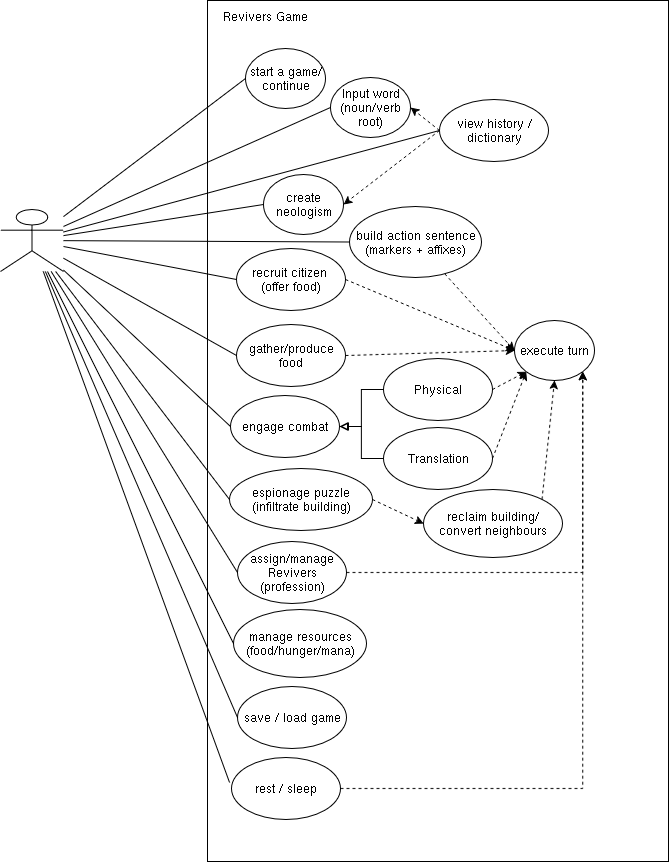
\includegraphics[width=0.7\textwidth]{../images/usecase.png}
  \caption{Use-case diagram.}
  \label{fig:usecase}
\end{figure}

\subsubsection{Activity Diagram}

\begin{figure}[H]
  \centering
  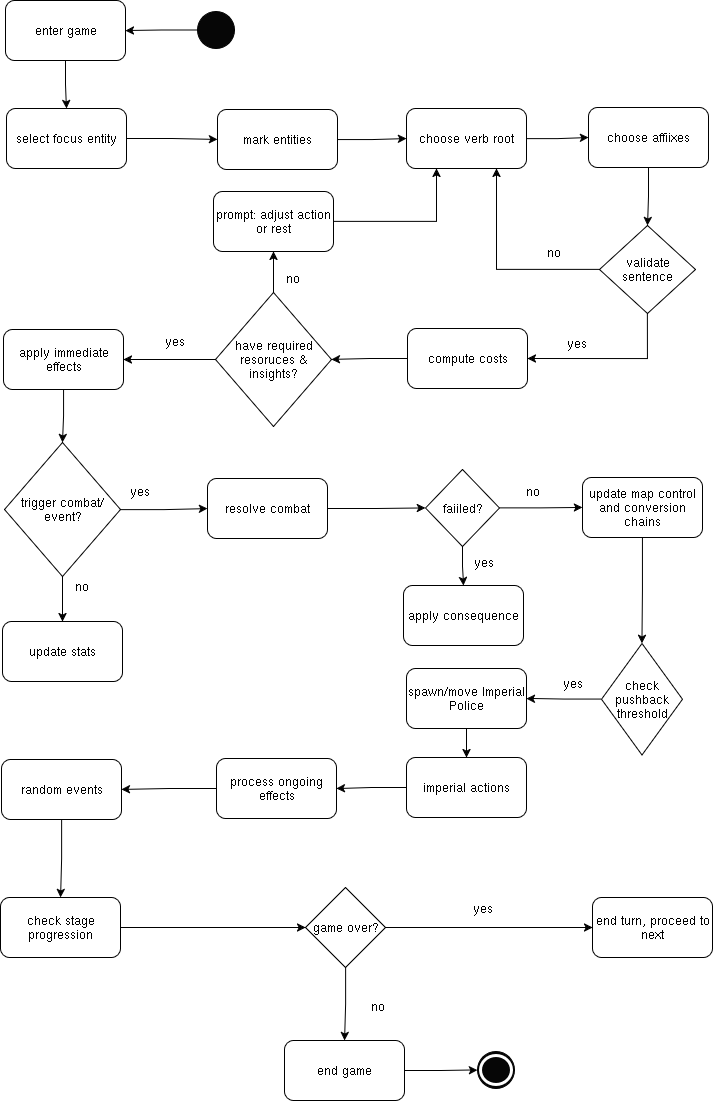
\includegraphics[width=0.7\textwidth]{../images/act.png}
  \caption{Activity diagram.}
  \label{fig:act}
\end{figure}

\subsubsection{Data Diagram}

\begin{figure}[H]
  \centering
  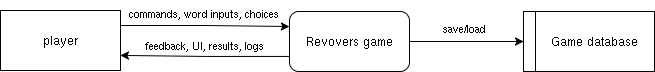
\includegraphics[width=0.7\textwidth]{../images/dfd0.png}
  \caption{Context diagram.}
  \label{fig:dfd0}
\end{figure}

\begin{figure}[H]
  \centering
  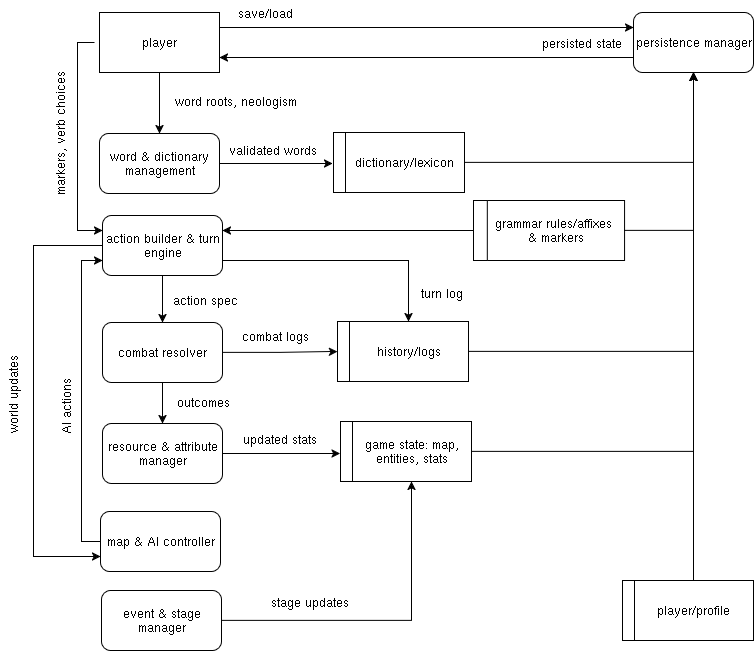
\includegraphics[width=0.7\textwidth]{../images/dfd1.png}
  \caption{Major processes and stores.}
  \label{fig:dfd1}
\end{figure}

\begin{figure}[H]
  \centering
  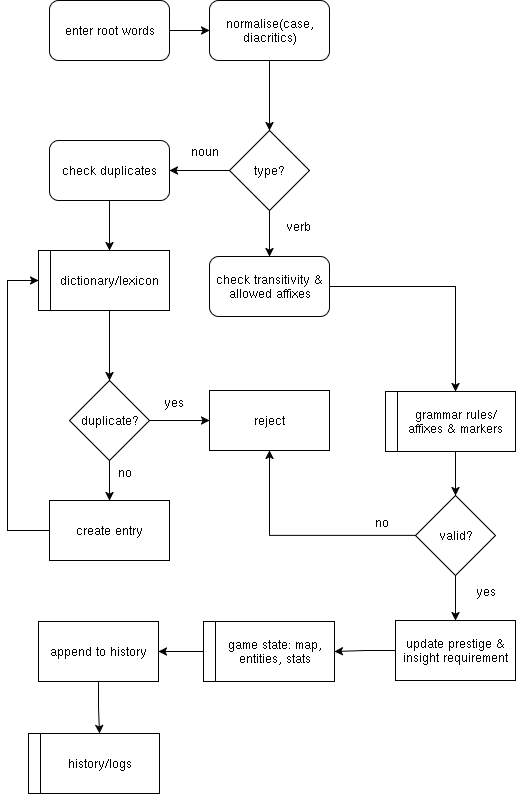
\includegraphics[width=0.7\textwidth]{../images/dfd2a.png}
  \caption{Word submission and validation diagram.}
  \label{fig:dfd2a}
\end{figure}

\subsection{Features and Functionalities}
The game will use entity-component-system structure in its design. Entities are the nouns in the game such as units, buildings and resources. Components are the data attached to these entities. Systems are the logic that operates on these entities with certain components.

\subsubsection{Core Gameplay}
\textbf{Entities}:
\begin{itemize}
\item
  Player
\item
  Revivers
\item
  Citizens
\item
  Imperial Police
\item
  Imperial Guards
\item Buildings
\item
  words (as collectible entities)
\end{itemize}

\textbf{Components}
\begin{itemize}
\item
  TurnComponent: action points, currentPhase
\item
  StageComponent: progress, unlockedFeatures
\item
  ActionComponent: chosen action plus arguments
\item
  AspectComponent: perfective, imperfective, contemplative
\end{itemize}

\textbf{Systems}
\begin{itemize}
\item
  TurnSystem: reset action points, start turns
\item
  ActionSystem: executes player actions
\item
  AISystem: NPC moves
\item
  StageSystem: check conditions and unlock mechanics
\item
  AspectSystem: resolve effects over time
\end{itemize}

\subsubsection{Player Management}
\textbf{Entities}:
\begin{itemize}
\item
  Player
\end{itemize}

\textbf{Components}
\begin{itemize}
\item
  ProfileComponent: name, ID
\item
  ResourceComponent: food, prestige, mana, hunger
\item
  ProgressComponent: stage, victories, defeats
\end{itemize}

\textbf{Systems}
\begin{itemize}
\item
  ResourceSystem: update resources
\item
  WinConditionSystem: check victory or defeat
\item
  PersistenceSystem: save and load profilees
\end{itemize}

\subsubsection{NPC and AI}
\textbf{Entities}:
\begin{itemize}
\item
  NPCEntity: citizen, revivers, guard, police, spy
\end{itemize}

\textbf{Components}
\begin{itemize}
\item
  EvenTriggerComponent
\item
  RelationComponent: loyalty hostility
\item
  AIComponrnt: decision state
\end{itemize}

\textbf{Systems}
\begin{itemize}
\item
  AISystem: generate decisions
\item
  RelationSystem: update trust, hostility
\item
  EventSystem: spawn resistance, recruitable events
\item
  Camera System: moves the camera one tile at a time across the map grid
\end{itemize}

\subsubsection{World and Data}
\textbf{Entities}:
\begin{itemize}
\item
  WorldEntity: map, dictionary, language DB
\end{itemize}

\textbf{Components}
\begin{itemize}
\item
  MapComponent: tiles, ownership
\item
  DictionaryComponent: player's collected words
\item
  LanguageDataComponent: words, roots, affixes
\item
  LogComponent: past actions
\end{itemize}

\textbf{Systems}
\begin{itemize}
\item
  LogSystem:append action outcomes
\item
  PersistenceSystem: save and load world
\item
  DictionarySystem: store and validate words
\item
  WorldSystem: manages global map state
\item
  TurnSystem: manages the selection of nouns and verbs during actions.
\end{itemize}

\subsubsection{UI/UX}
\textbf{Entities}:
\begin{itemize}
\item
  UIEntity: HUD, Dashboard, DialogueBox
\end{itemize}

\textbf{Components}
\begin{itemize}
\item
  RenderComponent: sprites, HUD text
\item
  DialogueComponent: npcID, text
\item
  PopupComponent: eventID
\end{itemize}

\textbf{Systems}
\begin{itemize}
\item
  RenderSystem: map and UI
\item
  HUDSystem: update resources, stage, influence
\item
  DialoogueSystem: display NPC text
\item
  EventUISystem: show popups
\end{itemize}

\subsubsection{System/Meta}
\textbf{Entities}:
\begin{itemize}
\item
  TutorialEntity
\item
  SettingsEntity
\end{itemize}

\textbf{Components}
\begin{itemize}
\item
  TutorialComponent: stageID, progress
\item
  SettingComponent: language, difficulty
\end{itemize}

\textbf{Systems}
\begin{itemize}
\item
  TutorialSystem: display guidance
\item
  SettingsSystem: change settings values
\item
  PersistenceSystem: database/file storage
\end{itemize}


\subsection{Timeline and Development Milestones}
This is the timeline for the development of the game done written in org-mode Emacs and turned into Gantt chart using elgantt-mode. The dates are under possible changes in the future.\\

\begin{figure}[H]
  \centering
  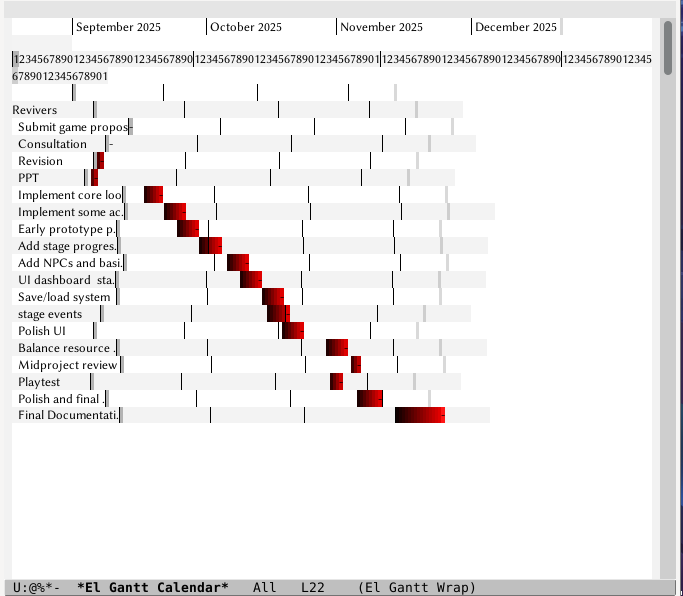
\includegraphics[width=0.7\textwidth]{../images/elgantt.png}
  \caption{Tentative developmental timeline.}
  \label{fig:gantt}
\end{figure}


\end{document}
